This section details our experimental methodology and the  video  datasets used. We evaluate our approach on the two popular datasets
Youtube Action Dataset and the Olympic Sports dataset. On both datasets, we show that our work exceeds the current state-of-the-art
results, by comparing with other popular techniques. Also, we vary the contribution of static and motion features, for the calculation
of combined vector series, and explore what is optimum contribution from each domain. By this step, we also prove that both static and motion features
are complementery, and provide vital information about the actions occuring in a video. Furthemore, we highlight the importance of considering the time evolution
of sub activities, in order to identify a complex event, by comparing the results of RNN and other methodologies, which does not capture
the temporal dynamics. 

\subsection{Datasets}
\noindent
\textbf{Holywood 2}: It consists of 12 classes of human actions distributed over 1500 video clips:
\textit{Answer phone, drive car, eat, fight person, get out car, hand shake, 
hug person, kiss, run, sit down, sit up, }and \textit{stand up}.
The dataset is composed of video clips from 69 movies and provides a challenging task, in automatic action detection.

\noindent
\textbf{UCF-11}: It consists over 1000
sports and home videos from YouTube. This dataset contains 11 action classes: 
\textit{basketball shooting, cycle, dive, golf swing, horse
back ride, soccer juggle, swing, tennis swing, trampoline
jump, volleyball spike}, and \textit{walk with a dog}. Each of the action 
sets is subdivided into 25 groups sharing similar environment conditions. 
This also is a challenging dataset with
camera jitter, cluttered backgrounds and variable illumination. 


\subsection{Contribution of Static and Motion domains}

The derivation done in section 4, for fusioning the static and motion vectors,
provides us a insightful intuition. That is, we can controll the contribution
of motion and static domains, to the fusion vector, by varying the $\rho$ value. 
The derivation of $\rho$ values for different contribution ratios, is illustrated in 
\ref{tbl:rho change}

\begin{table}
  
\begin{center}
  \begin{tabular}{ | l | c | r | }
    \hline
    \textbf{Contribution to $Z$} & \textbf{$\rho$ value} & \textbf{Fusion vector} \\ \hline
    {\makecell{ 80\% Motion, 20\% Static \\ $\rho_{1}=4\rho_{2}$ }} & \makecell{$\frac{1}{4}\rho_{1}=\sqrt{1-\rho_{1}^2}$ \\ $\rho_{1} = \frac{4}{\sqrt{17}}$} & $Z=\frac{4}{\sqrt{17}}M + \frac{1}{\sqrt{17}}S$ \\ \hline
    {\makecell{ 60\% Motion, 40\% Static \\ $2\rho_{1}=3\rho_{2}$ }} & \makecell{$\frac{2}{3}\rho_{1}=\sqrt{1-\rho_{1}^2}$ \\ $\rho_{1} = \frac{3}{\sqrt{13}}$} & $Z=\frac{3}{\sqrt{13}}M + \frac{2}{\sqrt{13}}S$ \\ \hline
    {\makecell{ 40\% Motion, 60\% Static \\ $3\rho_{1}=2\rho_{2}$ }} & \makecell{$\frac{3}{2}\rho_{1}=\sqrt{1-\rho_{1}^2}$ \\ $\rho_{1} = \frac{2}{\sqrt{13}}$} & $Z=\frac{2}{\sqrt{13}}M + \frac{3}{\sqrt{13}}S$ \\ \hline
     {\makecell{ 60\% Motion, 40\% Static \\ $4\rho_{1}=\rho_{2}$ }} & \makecell{$4\rho_{1}=\sqrt{1-\rho_{1}^2}$ \\ $\rho_{1} = \frac{1}{\sqrt{17}}$} & $Z=\frac{1}{\sqrt{17}}M + \frac{4}{\sqrt{17}}S$ \\ \hline
      \label{tbl:rho change}
  \end{tabular}
\end{center}
\caption{Derivation of contribution of static and motion domains to the fusion vector}
\end{table}

Results, for these $\rho$ values, for UCF-11 and Hollywood2 datasets, are shown in table and table, respectively. 
We use accuracy and mean average precision as performance matrics, for UCF-11 and 
Hollywood2, respectively.

\begin{table}[]
\centering
\caption{My caption}
\label{my-label}
\begin{tabular}{|l||l|l|l|l|l|}
\hline
Class            & rho & rho & rho & rho & rho \\ \hline  \hline
B shooting       &     &     &     &     &     \\ \hline
Biking           &     &     &     &     &     \\ \hline
Diving           &     &     &     &     &     \\ \hline
G swinging       &     &     &     &     &     \\ \hline
H riding         &     &     &     &     &     \\ \hline
S juggling       &     &     &     &     &     \\ \hline
Swinging         &     &     &     &     &     \\ \hline
T swinging       &     &     &     &     &     \\ \hline
T jumping        &     &     &     &     &     \\ \hline
V spiking        &     &     &     &     &     \\ \hline
W dog            &     &     &     &     &     \\ \hline \hline
Overall Accuracy &     &     &     &     &     \\ \hline
\end{tabular}
\end{table}

\begin{table}[]
\centering
\caption{My caption}
\label{my-label}
\begin{tabular}{|l|l|l|l|l|l|}
\hline
Class            & rho & rho & rho & rho & rho \\ \hline
AnswerPhone       &     &     &     &     &     \\ \hline
DriveCar           &     &     &     &     &     \\ \hline
Eat           &     &     &     &     &     \\ \hline
FightPerson         &     &     &     &     &     \\ \hline
GetOutCar       &     &     &     &     &     \\ \hline
HandShake        &     &     &     &     &     \\ \hline
HugPerson       &     &     &     &     &     \\ \hline
Kiss        &     &     &     &     &     \\ \hline
Run        &     &     &     &     &     \\ \hline
SitDown           &     &     &     &     &     \\ \hline
SitUp           &     &     &     &     &     \\ \hline
StandUp           &     &     &     &     &     \\ \hline
mAP          &     &     &     &     &     \\ \hline
\end{tabular}
\end{table}

Also, an overview distribution of the overall performance, over $\rho$ values, for both datasets, is shown in table.
We can see that, the performance change, for different contribution precentages of motion and static domain. Also, the optimum contribution may change
depending on the nature of the data. For example, if the motion patterns are indistinguishable accross actions, static information plays 
a critical role, for determining the action, and vise versa. This highilghts
our hypothesis, that being able to control this contibution explcitly, is vital for an action recognition system. 









\subsection{Comparison with the state-of-the-art}

able 2 compares our results to state of the art. $\rho = \frac{1}{\sqrt{2}}$ is used to combine the static and motion vectors,
since it gave the best results, for this dataset. On UCF-11, we significantly outperform 
the state of the art \cite{} by \%. A mean average precision of \% is achieved by our system, which outperforms
the state-of-the-art by \%. 

\begin{table}[]
\centering
\caption{My caption}
\label{my-label}
\begin{tabular}{|l|l||l|l|}
\hline
\multicolumn{2}{|c||}{UCF-11}    & \multicolumn{2}{c|}{Hollywood2} \\ \hline
Liu et al.            & 71.2\%  & Vig al.           & 59.4\%      \\ \hline
Ikizler-Cinbis et al. & 75.21\% & Jiang et al.      & 59.5\%      \\ \hline
Dense trajectories    & 84.2\%  & Mathe al.         & 61.0\%      \\ \hline
Sameera et al         &         & Jain al           & 62.5\%      \\ \hline
                      &         & Dense             & 58.3\%      \\ \hline
                      &         & Improved          & 64.3\%      \\ \hline \hline
Our method            &         & Our method        &             \\ \hline
\end{tabular}
\end{table}



\begin{table*}[]
\centering
\caption{My caption}
\label{my-label}
\begin{tabular}{|l||l|l|l|l|l|}
\hline
Class            & Ours & KLT & Wang et al. & kizler-Cinbis & Sameera et. al. \\ \hline  \hline
B shooting       &     &     &     &     &     \\ \hline
Biking           &     &     &     &     &     \\ \hline
Diving           &     &     &     &     &     \\ \hline
G swinging       &     &     &     &     &     \\ \hline
H riding         &     &     &     &     &     \\ \hline
S juggling       &     &     &     &     &     \\ \hline
Swinging         &     &     &     &     &     \\ \hline
T swinging       &     &     &     &     &     \\ \hline
T jumping        &     &     &     &     &     \\ \hline
V spiking        &     &     &     &     &     \\ \hline
W dog            &     &     &     &     &     \\ \hline \hline
Overall Accuracy &     &     &     &     &     \\ \hline
\end{tabular}
\end{table*}

\begin{table*}[]
\centering
\caption{xsfsdfsdf}
\label{my-label}
\begin{tabular}{|l|l|l|l|l|l|}
\hline
Class            & Ours & KLT & Wang et al. & Ullah   \\ \hline \hline
AnswerPhone       &     &     &     &         \\ 
DriveCar           &     &     &     &      \\ 
Eat           &     &     &     &          \\
FightPerson         &     &     &     &          \\ 
GetOutCar       &     &     &     &        \\ 
HandShake        &     &     &     &          \\ 
HugPerson       &     &     &     &          \\ 
Kiss        &     &     &     &          \\ 
Run        &     &     &     &          \\ 
SitDown           &     &     &     &          \\ 
SitUp           &     &     &     &          \\ 
StandUp           &     &     &     &          \\ \hline
mAP          &     &     &     &          \\ \hline
\end{tabular}
\end{table*}




Per action class results, are also compared in table and table. In UCF-11, our method excells
in 8 out of 11 classes, when compared with \cite{}, \cite{}, \cite{} and \cite{} We only fall behind in asd and asda classes. In Hollywood2,
we calculate the average precision of each class, and compare with \cite{}, \cite{}, \cite{} and \cite{}.
We achieve best results in 8 out of 12 classes in this case. 






\subsection{Effectiveness of Capturing Time Evolution}
As discussed in earliar sections, complex actions are composed of sub activities, preserving
a temporal pattern. In this work, we try to capture those underlying patterns, by a LSTM netwok.
It is interesting to verify, whether this stratergy has an impact on the accuracy of the 
classification. Here, we directly feed the fused vectors to a random forest classifier, which
does not capture sequencial dynamic patterns, and compare it with the results obtained by
the LSTM network. The results are shown in table

As indicated by the results in chart, LSTM network significantly outperforms the 
random forest classifier, for both datasets. Therefore, it can be concluded that, exploiting 
temporal patterns of sub activities, benifits complex action classification. 



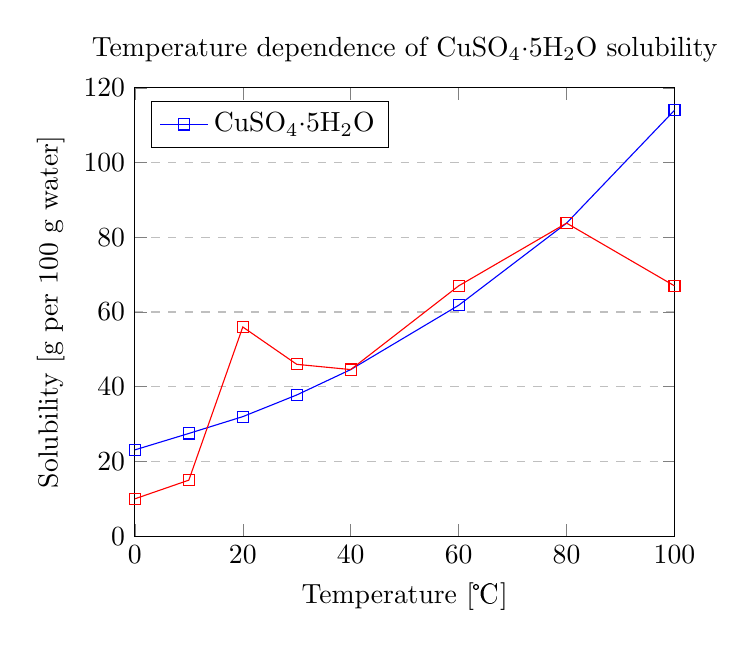
\begin{tikzpicture}
\begin{axis}[
    title={Temperature dependence of CuSO$_4\cdot$5H$_2$O solubility},
    xlabel={Temperature [\textcelsius]},
    ylabel={Solubility [g per 100 g water]},
    xmin=0, xmax=100,
    ymin=0, ymax=120,
    xtick={0,20,40,60,80,100},
    ytick={0,20,40,60,80,100,120},
    legend pos=north west,
    ymajorgrids=true,
    grid style=dashed,
]
 
\addplot[
    color=blue,
    mark=square,
    ]
    coordinates {
    (0,23.1)(10,27.5)(20,32)(30,37.8)(40,44.6)(60,61.8)(80,83.8)(100,114)
    };
    \legend{CuSO$_4\cdot$5H$_2$O}
    
    \addplot[
    color=red,
    mark=square,
    ]
    coordinates {
    (0,10)(10,15)(20,56)(30,46)(40,44.6)(60,67)(80,83.8)(100,67)
    };
    \legend{CuSO$_4\cdot$5H$_2$O}
\end{axis}
\end{tikzpicture}



